%Her beskrives kort hvordan projektets HW-dele og SW-dele er implementeret (”lavet”). HW-delene kan med fordel beskrives med få, udvalgte, tydelige fotos. Her beskrives også kort hvordan SW-delene er implementeret (kodet). Den/de anvendte compilere beskrives meget kort (programmeringssprog, version etc.). Der argumenteres for valg af programmeringssprog. Der vises kun source code i projektrapporten, når der er tale om ekstremt interessante, små kodeudsnit. Der henvises til projektets bilag, hvor relevante/tydelige fotos af projektets HW og den samlede source code for projektets SW er anbragt.
\chapter{Implementation}
In this section, the implementation of Captain system will be discussed. This includes mechanical and electronic hardware choices, as well as software choices.
More detailed descriptions of everything discussed in this section can be found in the documentation in section~\ref{sec:implementation}, on page~\pageref{sec:implementation}.

\section{Hardware}
There are two types of hardware in this project, mechanical and electronic. The mechanics are the boat, rudder, thruster and so on. The electronics are motor driver, power regulator and so forth. Only the electronics will be discussed, since the mechanics are already implemented as a boat.

\subsection{Electronics}
All of the electrical components of the system were connected on a perfboard\cite{perfboard}. The perfboard is used to distribute the power from the battery to voltage regulators. The signals from the Raspberry Pi are also routed through the perfboard to the servo and the motor controller. All of the signals are routed through detachable wires, to make it easy to measure and rearrange in case something requires signal testing or debugging. This perfboard system can be seen in figure~\ref{fig:integration}. 

\begin{figure}[H]
\centering
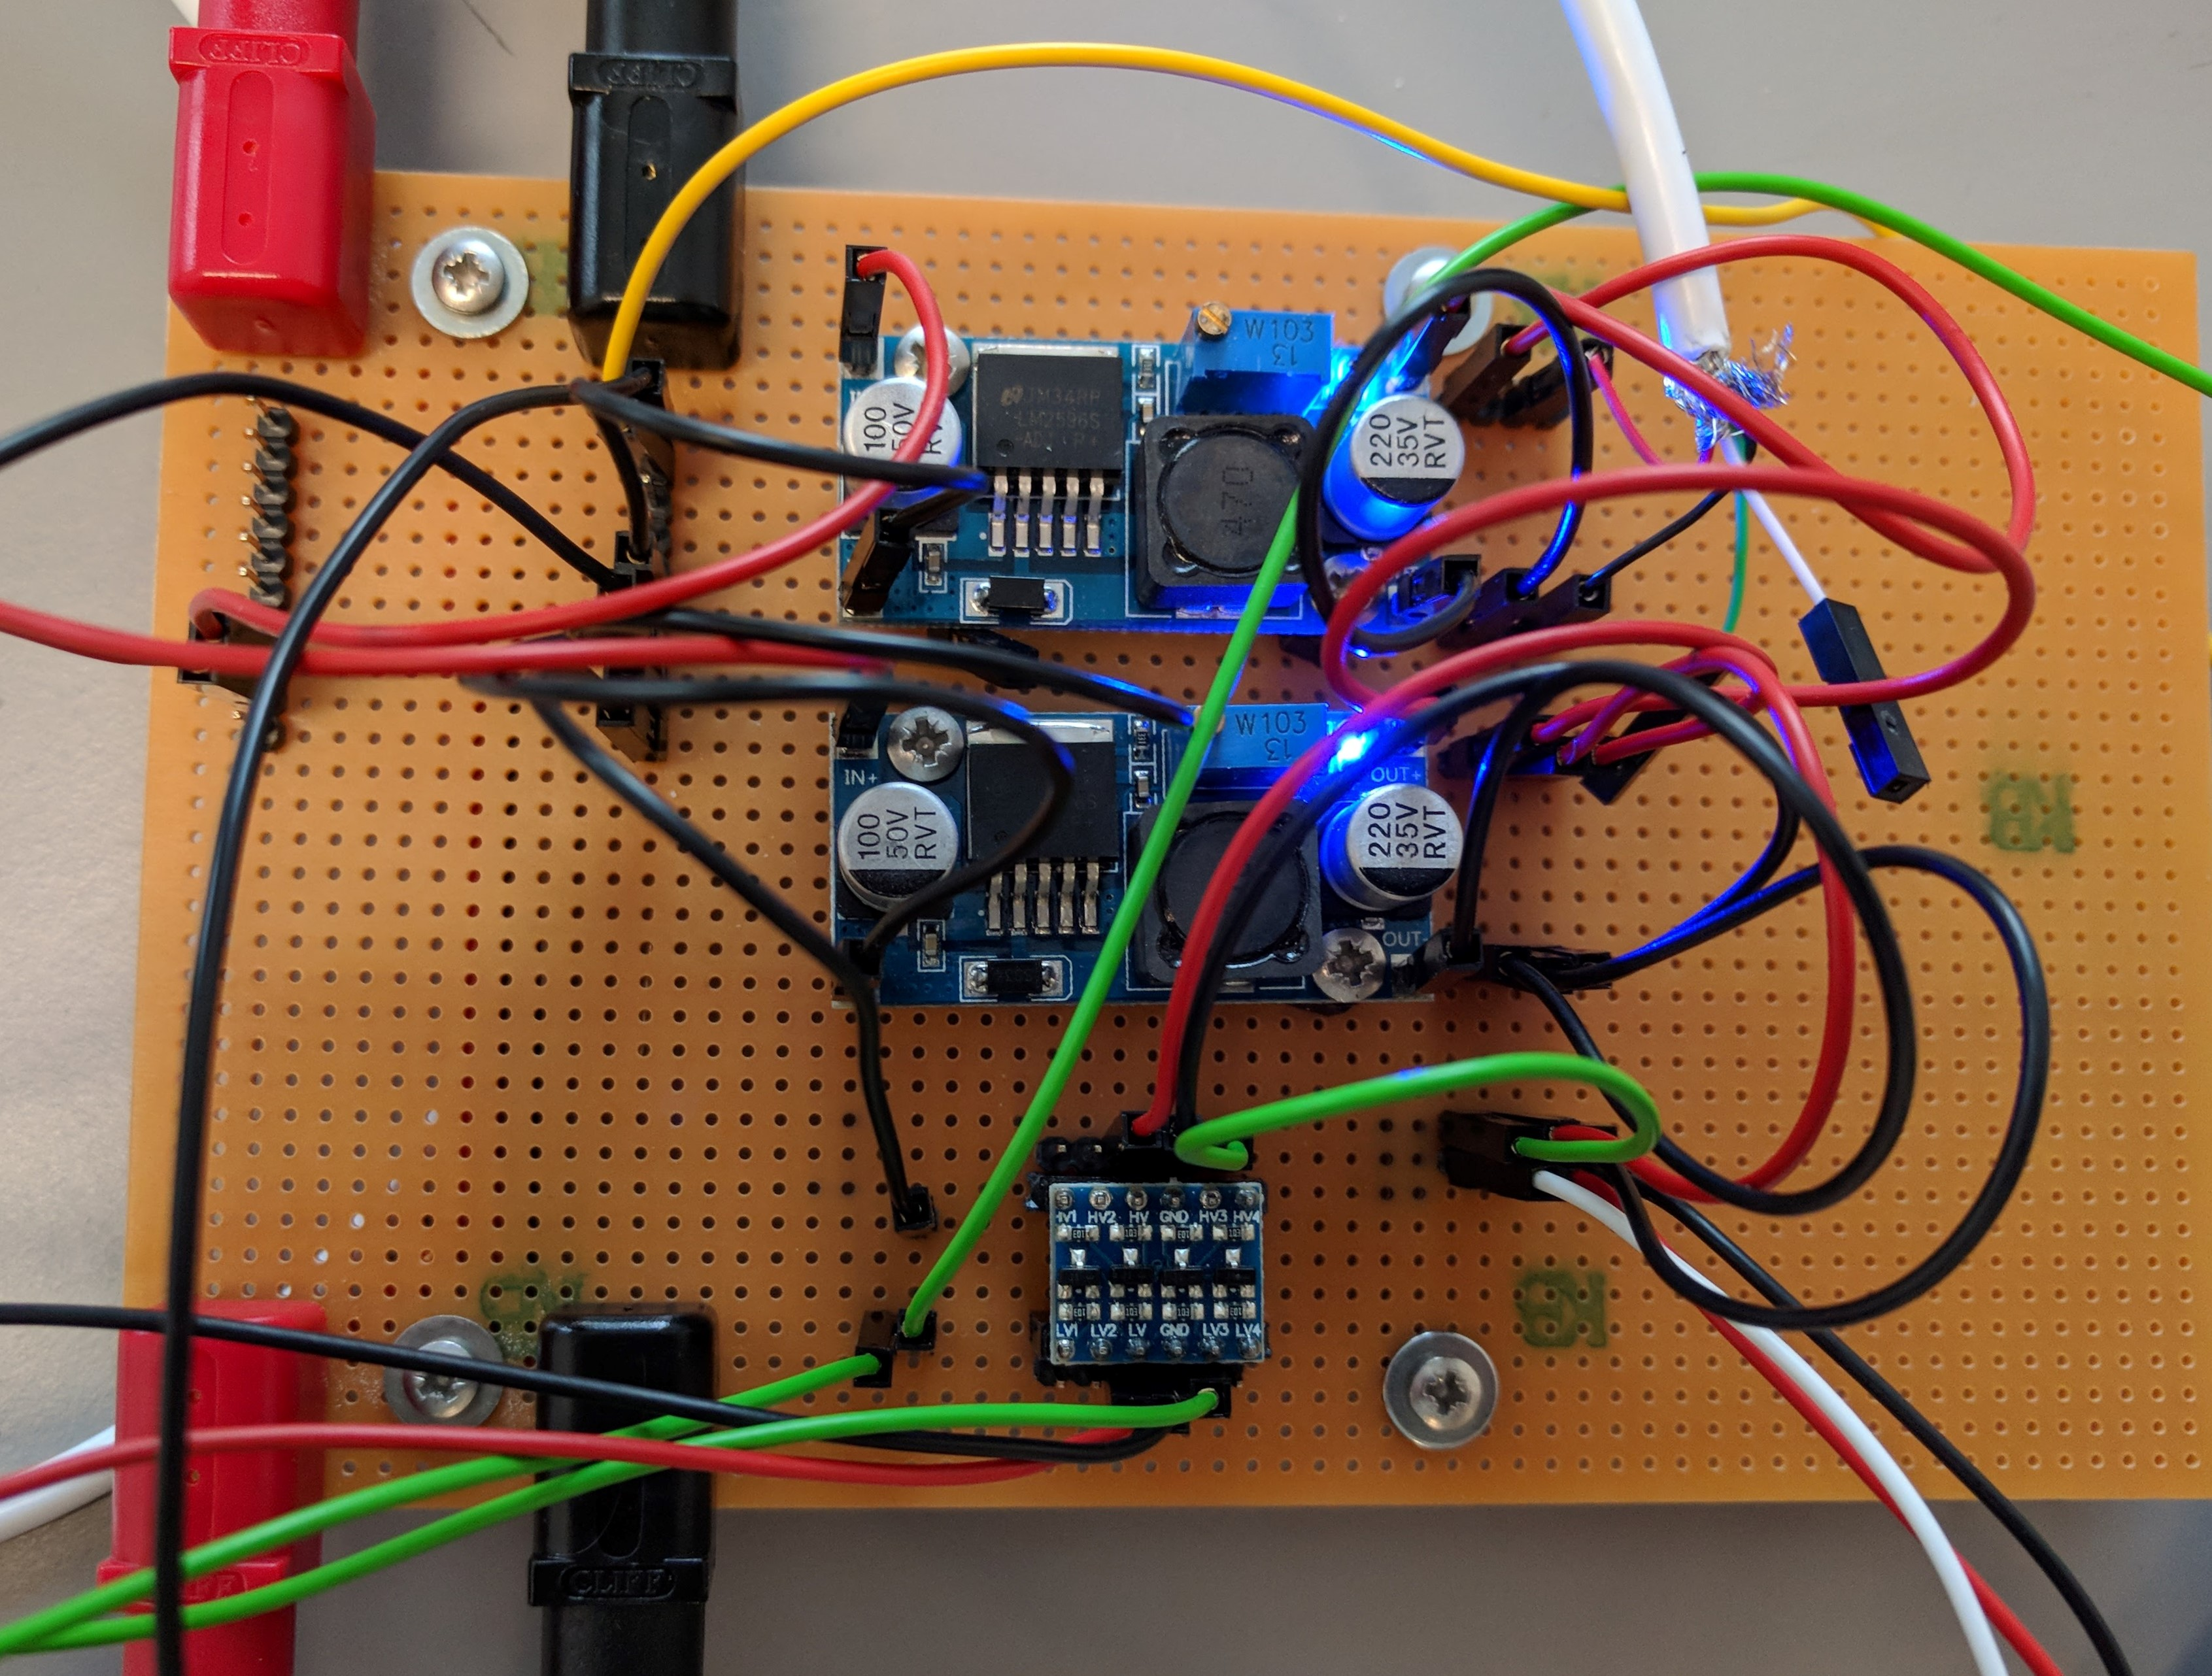
\includegraphics[width=0.7\linewidth]{../Appendix/Project/Dokumentation/Images/Implementation/integration}
\caption{Perfboard, used to connect all components}
\label{fig:integration}
\end{figure}

\section{Software}
In this section, the choices of compilers and programming languages will be discussed. The concrete code implementation will also be looked at from a very general standpoint.

\subsection{Programming languages}
This system is built up of two distinct parts in terms of software. There is the website user interface, and then there is the controller or what could be thought of as the backend. The website user interface is marked up in HTML and CSS with the help of the Bootstrap framework \cite{bootstrap}. In terms of code, JavaScript was used with AngularJS as a framework. 

For the other part of the system, the controller. C++ was the language of choice. This was simply because the development team has familiarity with this language. C++ has the advantage of being a very fast, but the drawback of having a rather low abstraction level. 
 
\subsection{Compiler}
For the website there is no real compiler since JavaScript is an interpreted language. But the server that runs the website is a Node.js server. Node.js is built on the Chrome V8 javascript engine at runtime. The client browser used to display the website was a Chrome web browser which is also built on the Chrome V8 javascript engine. 

The controller is written in C++ and is therefore compiled, the compiler used while developing the system was the was VS 2017 C++ Build tools\cite{VC-2017}. The compiler used on the Raspberry Pi is GCC 6.3.0 for raspbian\cite{GCC}. They are both C++11 compatible which made some things easier while developing. 

\subsection{Code}
%To start with lets have a look at the controller code. It is broken up just like the design states. 

One of the key components of the system is the GPS receiver, it is the sensor responsible for locating the boat. The controller has a class called Ublox\_neo7m, it is an implementation of the IGPS interface. The Ublox\_neo7m class gets its data by setting up a thread, which continually reads on a serial interface. The data from the serial interface is written to the correct variables. Any other part of the system can get data from the GPS receiver be it, status data such as fix and horizontal dilution of precision, or the pose of the boat. 

There is a thruster in the system as well, it is a DC-motor, which can be controlled by a PWM signal. Therefore the implementation of the class DCMotor uses an object of type IGPIO to send out PWM signals, where IGPIO is an interface that describes a general purpose I/O driver for a system. In this case it is for the Raspberry Pi and the PiGpio library is used\cite{pigpio}. It allows for the motor to set a hardware PWM to a frequency of 30 kHz and a wide spectrum of duty cycles.

As the thruster, the rudder class, called Servo, also uses an IGPIO interface to send PWM signals to a GPIO pin. The servo can set the position between 0\% and 100\%. In reality, the servos full range of motion is described as period of between 500 µs and 2500 µs, and a PWM frequency of 50 Hz. So the Servo class converts from one input to the other, it also uses the PiGpio built in function called GpioServo. Both the rudder and thruster is in controlled by the autopilot.

The Autopilot is in essence built up of two PID loops, one for the rudder, and one for the thruster. In the current implementation, it allows for the user to change the PID terms for the rudder PID loop through the user interface. The autopilots gets the data for what to do from the navigation class.

The Navigation class is responsible for perform tasks given by the user; calculating paths, and starting/stopping. To do this, it uses a number of algorithms, calls the GPS for new data, and finally transmits data back to the user as well as sending data to the autopilot if a path is being traversed.

The two path types used in this project are a simple line to a destination called a "point to point" path, and a more complicated "coverage rectangle" which, as the name implies, covers an area.

So for our project, the goal is not to get from A to B as quickly as possible, but to be able to map an area of the sea and give the user/client an intuitive user interface to input the desired area to map. For this reason, rhumb lines were chosen over great circle lines to represent lines on the globe, for more information see the documentation, section~\ref{sec:software_implementation} on page~\pageref{sec:software_implementation}.

The navigation unit uses the GeographicLib library to calculate rhumb lines and rhumb distances. Initially, an algorithm was written by the devleopment team to do this, but after comparing it to the one offered in the Geographic library, the performance and precision was much better, and it was decided to use the library for these two functions, and for importing the WGS84 constants. All other Navigation algorithms and calculations have been designed, developed, and tested by the project team.

How the algorithms in the Navigation unit work can be seen in the documentation, section~\ref{sec:software_implementation} on page~\pageref{sec:software_implementation}.

The navigation uses the JSONTrasmitter to send data to the user interface.

The ITransmitter interface is implemented as one transmitter; JSONTransmitter. This class is responsible for collecting information from the motors, navigation, and gps modules, translate it to valid JSON format, and then update the fromNav.json file. To handle JSON format parsing in C++, the "JSON for modern C++" library by Niels Lohmann was used\cite{json}. 

The Transmitter is called by the Navigation when a task has been performed, and is given a timestamp. It then collects NavigationData from the Navigation class, MotorStatuses from the two motors, and a GPSStatus from the gps. From this it builds a JSON "tree" of objects, and packages them correctly, taking edge cases into account, as defined by the fromNav.json protocol. 

In the other end of the system, the JSONReceiver is responsible for receiving data from the files as the name implies.

To receive data from the user interface, a JSONReceiver has been implemented, as an implementation of the IReceiver interface. The receiver is in charge of reading two files that reside in the website. One is the toNav.json file, and the other is the activeParam.json. toNav.json is the file that holds the current command from the website, this could be to calculate a path with a certain rectangle defined. The JSONReceiver then takes this command and data it has been given and passes it on to the navigation through the perform task function. The other file, activeParam.json, holds the currently activated parameter profile from the user. The data it gets from this file is passed and then passed on to the appropriate classes, i.e. either the autopilot or the navigation.

The data that is read or received from the JSONReciever comes from the user interface, which is made up of two parts, a website user interface, that can be opened in the browser, and a Node.js server that hosts the website. 

The website has four pages, point to point, coverage, status, and edit parameter. The point to point page allows the user to enter one point for the boat to travel to. When the user presses the calculate button, the website sends a POST call to the server hosting it. This then sends a command with information about the current position and desired target for the calculation to the JSONReceiver. Then it gets a path back from the JSONTransmitter from the fromNav.json file, and the path is displayed. The user can now press start, and the start command is sent. Back from the JSONTransmitter comes the progress of completing the path. This sequence is exactly the same for the coverage page, except that it takes two points to define the rectangle start- and endpoints. 

The status page on the website has one responsibility which is parsing the status object that is in the fromNav.json file. This object contains diagnostics data for several parts of the system. The status page dynamically runs through all these items and displays them on the screen.

Lastly on the website there is the edit parameter page, and this is where the technician setup to boat with all of the parameters that can be modified. It does this by letting the user create, delete and edit JSON objects in a list. This list is saved on the server, along with the currently active parameter profile. 

As mentioned before the user interface is hosted on a Node.js server\cite{nodejs}. This is what is responsible for handling POST calls from the website. All of the POST calls it is setup to handle is for saving data to a file, so both the website and the controller can read it.

%GPS
%Servo / Motor
%Autopilot
%Navigation
%Transmitter
%Reciever
%Hjemme side


%Software
%%compilere
%%Programmeringsprog + argumentation
%%Kode
